%&pdflatex
\documentclass[mathserif]{beamer} %, handout
\usetheme[progressbar=foot]{metropolis}
\setbeamertemplate{caption*}[numbered]

\usepackage[utf8x]{inputenc}
\usepackage[T2A]{fontenc}
\usepackage[english,russian]{babel}

\usepackage{amssymb, amsmath, amsfonts, mathtools, mathrsfs}
\usepackage[normalem]{ulem} % for sout
\usepackage{comment}

\usepackage{subcaption}
\usepackage{tikz}
\usepackage{pgfplots}

\title{Численный анализ медленных неизотермических течений слаборазреженного газа}
\author{Рогозин Олег Анатольевич}
\institute{
    Вычислительный центр ФИЦ ИУ РАН
}
\date{}

\newcommand{\Kn}{\mathrm{Kn}}
\newcommand{\St}{\mathrm{St}}
\newcommand{\Ma}{\mathrm{Ma}}
\newcommand{\loc}{\mathrm{loc}}
\newcommand{\eqdef}{\overset{\mathrm{def}}{=}}
\newcommand{\dd}{\:\mathrm{d}}
\newcommand{\pder}[2][]{\frac{\partial#1}{\partial#2}}
\newcommand{\pderdual}[2][]{\frac{\partial^2#1}{\partial#2^2}}
\newcommand{\pderder}[3][]{\frac{\partial^2#1}{\partial#2\partial#3}}
\newcommand{\Pder}[2][]{\partial#1/\partial#2}
\newcommand{\dxi}{\dd\xi}
\newcommand{\OO}[1]{O(#1)}
\newcommand{\Set}[2]{\{\,{#1}:{#2}\,\}}
\newcommand{\xoverbrace}[2][\vphantom{\int}]{\overbrace{#1#2}}
\newcommand{\Cite}[2][]{\alert{\textsc{#2 #1}}}
\newcommand{\inner}[2]{\left\langle{#1},{#2}\right\rangle}
\newcommand{\onwall}[1]{\left(#1\right)_0}
\newcommand{\deltann}[2]{(\delta_{#1#2}-n_#1 n_#2)}


% use Russian tradition
\renewcommand{\phi}{\varphi}
\renewcommand{\epsilon}{\varepsilon}

\begin{document}

\frame{
    \begin{flushright}
        \textit{Памяти Оскара Гаврииловича Фридлендера (1939--2015)}
    \end{flushright}
    \vspace{-30pt}
    \titlepage
}

\begin{frame}
    \frametitle{Содержание}
    \linespread{0.8}
    \tableofcontents
\end{frame}

\section{Асимптотический анализ уравнения Больцмана}

\begin{frame}
    \frametitle{Разложение Гильберта для медленных течений}
    Стационарное уравнение Больцмана в присутствии внешней силы
    \begin{equation}\label{eq:Boltzmann}
        \xi_i\pder[f]{x_i} + F_i\pder[f]{\xi_i} = \frac1k J(f,f).
    \end{equation}
    Разложение по числу Кнудсена \(k=\Kn\sqrt\pi/2\):
    \begin{equation}\label{eq:expansion}
        f = f_0 + f_1k + f_2k^2 + \cdots, \quad h = h_0 + h_1k + h_2k^2 + \cdots,
    \end{equation}
    где макроскопические величины \(h = \rho, v_i, T, \dots\)
    \vspace{5pt}\pause

    Предположения:
    \begin{itemize}
        \item медленные течения \(v_i = \OO{k}\) (\(\mathrm{Re} = \OO{1}\))
        \item слабая внешняя сила \(F_i = \OO{k^2}\)
    \end{itemize}
    Из-за вырожденности уравнения движения
    \begin{equation}
        \pder[p_0]{x_i} = 0, \quad \pder[p_1]{x_i} = 0.
    \end{equation}
\end{frame}

\begin{frame}
    \frametitle{Уравнения гидродинамического типа}
    \Cite[1970, 1971, 1976]{Коган, Галкин, Фридлендер}:
    \begin{align*}
        \pder{x_i}\left(\frac{u_{i1}}{T_0}\right) &= 0, \\
        \pder{x_j}\left(\frac{u_{i1}u_{j1}}{T_0}\right)
            &-\frac12\pder{x_j}\left[\Gamma_1\left(
                \pder[u_{i1}]{x_j} + \pder[u_{j1}]{x_i} - \frac23\pder[u_{kH1}]{x_k}\delta_{ij}
            \right)\right] \notag\\
            &-\alert{\left[
                \frac{\Gamma_7}{\Gamma_2}\frac{u_{j1}}{T_0}\pder[T_0]{x_j}
                + \frac{\Gamma_2^2}4 \left(\frac{\Gamma_7}{\Gamma_2^2}\right)'
                    \left(\pder[T_0]{x_j}\right)^2
            \right]\pder[T_0]{x_i}} \notag\\
            &= -\frac12\pder[p_2^\dag]{x_i}, \\
        \pder[u_{i1}]{x_i} &= \frac12\pder{x_i}\left(\Gamma_2\pder[T_0]{x_i}\right),
    \end{align*}
    где
    \begin{equation*}
        p_2^\dag = p_0 p_2
            + \frac23\pder{x_k}\left(\Gamma_3\pder[T_0]{x_k}\right)
            - \frac{\Gamma_7}{6}\left(\pder[T_0]{x_k}\right)^2, \quad u_{i1} = p_0v_{i1}.
    \end{equation*}
\end{frame}

\begin{frame}
    \frametitle{Уравнения гидродинамического типа}
    \centering{\Large\bf Как их назвать?}
    \vspace{10pt}
    \begin{itemize}
        \item SNIF equations \Cite[1993]{Коган}, \Cite[1995]{Bobylev}
        \item ghost effect equations \Cite[2009]{Levermore+}, \Cite[2017]{Aoki+}
        \item уравнения Когана"--~Галкина"--~Фридлендера \Cite[2017]{Рогозин}
    \end{itemize}

    \centering{\Large\bf Экспериментальное подтверждение}
    \begin{itemize}
        \item \Cite[1997, 2003]{Friedlander, Nikolsky et al.}:\\
            в аэродинамической трубе ЦАГИ
    \end{itemize}
\end{frame}

\begin{frame}
    \frametitle{Действующие силы}
    Для степенного потенциала
    \[ \Gamma_{1,2}(T) = \gamma_{1,2}T^s, \quad \Gamma_3(T) = \gamma_3T^{2s},
        \quad \Gamma_7(T) = \Gamma_3' - \gamma_7T^{2s-1}. \]
    На единицу массы газа действует сила
    \begin{equation}\label{eq:gamma7_force}
        F_i = -\frac{\Gamma_7}{4p_H} \left(\pder[T_H]{x_j}\right)^2 \pder[T_H]{x_i} k^2 + \OO{k^3},
    \end{equation}
    Она вызывает \emph{нелинейное термострессовое течение}.
    \vspace{10pt}\pause

    Сила, действующая на равномерно нагретое покоящееся тело,
    \begin{multline}\label{eq:force:terms}
        p_0 \oint_S F_{i2} \dd{S} =
            - \overbrace{ \oint_S p_2^\dag n_i \dd{S} }^\text{pressure} \\
            + \underbrace{ \Gamma_1\oint_S \pder[u_{i1}]{x_j} n_j \dd{S} }_\text{viscosity}
            + \underbrace{ \frac{\Gamma_7}{2} \oint_S \left(\pder[T_0]{x_j}\right)^2 n_i \dd{S} }_\text{thermal-stress}.
    \end{multline}
\end{frame}

\begin{frame}
    \frametitle{Boundary conditions and Knudsen-layer correction}
    Решение = гидродинамическая часть + кнудсеновская часть (поправка) \\
    Макроскопические переменные \(h = h_0 + (h_1 + \alert{h_{K1}})k + \cdots\)

    Теоремы {\footnotesize \Cite[1982]{Маслова}; \Cite[1986]{Bardos, Caflisch, Nicolaenko}}:
    \begin{equation}
        f_K = \OO{\eta^{-\infty}}, \quad \eta = \frac{p_0}{T_{B0}}(x_i-x_{Bi})\frac{n_i}k
    \end{equation}
    Декомпозиция единственна!
    \pause

    Граничные условия и \(h_K\) получаются из решения одномерного линеаризованного уравнения
    Больцмана в полупространстве.\\
    Для модели твёрдых сфер и диффузного отражения:
    \begin{itemize}
        \item первый порядок \Cite[1989]{Ohwada, Sone, Aoki},
        \item второй порядок \Cite[2015]{Takata, Hattori}.
    \end{itemize}
\end{frame}

\begin{frame}
    \frametitle{Слой Кнудсена первого порядка}
    \begin{equation}
        \alert{T_0} = T_{B0}. \label{eq:bc_T0}
    \end{equation}

    \begin{gather}
        \frac{p_0}{T_{B0}}
            \begin{bmatrix} \alert{T_1} - T_{B1} \\ T_{K1} \\ T_{B0}^2\rho_{K1} \end{bmatrix} =
            \onwall{\pder[T_0]{x_j}} n_j \begin{bmatrix} d_1 \\ \Theta_1(\eta) \\ p_0\Omega_1(\eta) \end{bmatrix}, \\
        \left\{
        \begin{aligned}
            & \frac1{\sqrt{T_{B0}}}\begin{bmatrix} (\alert{u_{j1}} - u_{Bj1}) \\ u_{jK1} \end{bmatrix} \deltann{i}{j} =
                \onwall{\pder[T_0]{x_j}}\begin{bmatrix} k_0 \\ Y_0(\eta) \end{bmatrix}\deltann{i}{j}, \\
            & \alert{u_{j1}} n_j = 0.
        \end{aligned}
        \right.
    \end{gather}
    \vspace{-20pt}
    \begin{itemize}
        \item \(\eta\) "--- растянутая координата вдоль нормали
        \item \(\Theta_1, \Omega_1, Y_0 = \OO{\eta^{-\infty}}\)
        \item \(\onwall{\cdots}\) "--- значение на границе (\(\eta=0\))
    \end{itemize}
\end{frame}

\begin{frame}
    \frametitle{Слой Кнудсена второго порядка}
    \footnotesize
    \begin{equation*}
        \begin{aligned}
            \frac1{\sqrt{T_{B0}}}&
                \begin{bmatrix} (u_{j2} - u_{Bj2}) \\ u_{jK2} \end{bmatrix}\deltann{i}{j} = \\
            &- \left.\frac{\sqrt{T_{B0}}}{p_0}\onwall{\pder[u_{j1}]{x_k}} \deltann{i}{j}n_k
                \begin{bmatrix} k_0 \\ Y_0(\eta) \end{bmatrix} \quad\right\}\text{velocity jump}\\
            &- \left.\frac{T_{B0}}{p_0}\onwall{\pderder[T_0]{x_j}{x_k}} \deltann{i}{j}n_k
                \begin{bmatrix} a_4 \\ Y_{a4}(\eta) \end{bmatrix} \quad\right\}\text{thermal slip} \\
            &\left.\begin{aligned}
                &- \bar\kappa\frac{T_{B0}}{p_0}\onwall{\pder[T_0]{x_j}} \deltann{i}{j}
                \begin{bmatrix} a_5 \\ Y_{a5}(\eta) \end{bmatrix} \\
                &- \kappa_{jk}\frac{T_{B0}}{p_0}\onwall{\pder[T_0]{x_k}} \deltann{i}{j}
                \begin{bmatrix} a_6 \\ Y_{a6}(\eta) \end{bmatrix}
            \end{aligned} \quad\right\}\text{curvature terms}\\
            &- \left.\pder[T_{B1}]{x_j} \deltann{i}{j}
                \begin{bmatrix} K_1 \\ \frac12 Y_1(\eta) \end{bmatrix}. \quad\right\}\text{thermal creep}
        \end{aligned}\label{eq:boundary_u2t}
    \end{equation*}
    \vspace{-10pt}
    \begin{itemize}
        \item \(\kappa_{ij} = \kappa_1 l_i l_j + \kappa_2 m_i m_j\) is the curvature tensor, \(\bar\kappa = (\kappa_1+\kappa_2)/2\)
    \end{itemize}
\end{frame}

\begin{frame}
    \frametitle{Слой Кнудсена второго порядка}
    \footnotesize
    \begin{gather*}
        \begin{multlined}
            \frac1{\sqrt{T_{B0}}}
                \begin{bmatrix} (u_{j2} - u_{Bj2}) \\ u_{jK2} \end{bmatrix} n_j = \\
            - \frac{T_{B0}}{p_0}\left[ \onwall{\pderder[T_0]{x_i}{x_j}}n_i n_j
                + 2\bar\kappa\onwall{\pder[T_0]{x_i}}n_i \right]
                \begin{bmatrix} \frac12\int_0^\infty Y_1(\eta_0)\dd\eta_0 \\
                    \frac12\int_\infty^{\eta} Y_1(\eta_0)\dd\eta_0 \end{bmatrix}.
        \end{multlined}\label{eq:boundary_u2n}\\
        \begin{aligned}
            \frac{p_0}{T_{B0}}
                \begin{bmatrix} T_2 - T_{B2} \\ T_{K2} \\ T_{B0}^2\rho_{K2} \end{bmatrix}
            &= \onwall{\pder[T_1]{x_j}} n_j
                \begin{bmatrix} d_1 \\ \Theta_1(\eta) \\ p_0\Omega_1(\eta) \end{bmatrix} \\
            &+ \frac{T_{B0}}{p_0}\onwall{\pderder[T_0]{x_i}{x_j}} n_i n_j
                \begin{bmatrix} d_3 \\ \Theta_3(\eta) \\ p_0\Omega_3(\eta) \end{bmatrix} \\
            &+ \bar\kappa\frac{T_{B0}}{p_0}\onwall{\pder[T_0]{x_i}} n_i
                \begin{bmatrix} d_5 \\ \Theta_5(\eta) \\ p_0\Omega_5(\eta) \end{bmatrix}.
        \end{aligned}\label{eq:boundary_T2}
    \end{gather*}
\end{frame}

\section{Течение между некоаксиальными цилиндрами}

\begin{frame}
    \frametitle{Поле скоростей в континуальном пределе}
    \centering
    \begin{figure}
    \begin{overprint}
        \onslide<1| handout:2>
            \[ T_1 = 1, \quad T_2 = 5.\]
            \hspace{-1cm}
            \includegraphics[width=1.15\linewidth]{noncoaxial/cylinder5}
        \onslide<2| handout:1>
            \[ T_1 = 5, \quad T_2 = 1.\]
            \hspace{-1cm}
            \includegraphics[width=1.15\linewidth]{noncoaxial/inverse5}
        \onslide<3| handout:0>
            \[ T_1 = 1, \quad T_2 = 50.\]
            \hspace{-1cm}
            \includegraphics[width=1.15\linewidth]{noncoaxial/cylinder50}
    \end{overprint}
    \hspace{-.5cm}
    \end{figure}
\end{frame}

\begin{frame}
    \frametitle{Зависимость поля скоростей от \(\tau = T_2-T_1\)}
    \centering
    \begin{columns}
        \column{.7\textwidth}
        \begin{figure}
            \includegraphics[width=\linewidth]{noncoaxial/U-tau-cylinders}
            \vspace{-.5cm}\caption{максимальное значение скорости}
        \end{figure}
        \column{.4\textwidth}
        \[ u_{i1} = \OO{\tau^3}, \quad \tau\to0, \]
        \[ u_{i1} = \OO{\tau^{3/2}}, \quad \tau\to\infty. \]
    \end{columns}
\end{frame}

\begin{frame}
    \frametitle{Зависимость действующей силы от \(\tau = T_2-T_1\)}
    \vspace{-.2cm}
    \[ p_0 \oint_S F_{x2}\dd{S} = \OO{\tau^2}. \]
    \vspace{-.7cm}
    \begin{columns}
        \column{.6\textwidth}
        \begin{figure}
            \includegraphics[width=\linewidth]{noncoaxial/F-tau-cylinders-inner}
            \vspace{-.5cm}\caption{внутренний цилиндр}
        \end{figure}
        \column{.6\textwidth}
        \begin{figure}
            \includegraphics[width=\linewidth]{noncoaxial/F-tau-cylinders-outer}
            \vspace{-.5cm}\caption{внешний цилиндр}
        \end{figure}
    \end{columns}
\end{frame}

\begin{frame}
    \frametitle{Зависимость действующей силы от расстояния между осями}
    \vspace{-.5cm}
    \[ p_0 \oint_S F_{x2}\dd{S} = \begin{cases}
        \OO{(1-d)^{-1}} & \quad\text{для cфер}, \\
        \OO{(1-d)^{-3/2}} & \quad\text{для цилиндров}, \\
        \end{cases} \quad d\to1. \]
    \vspace{-.7cm}
    \begin{columns}
        \column{.6\textwidth}
        \begin{figure}
            \includegraphics[width=\linewidth]{noncoaxial/forces}
        \end{figure}
        \column{.6\textwidth}
        \begin{figure}
            \includegraphics[width=\linewidth]{noncoaxial/forces-close}
        \end{figure}
    \end{columns}
\end{frame}

\begin{frame}
    \frametitle{Электростатическая аналогия}
    \footnotesize
    Линейная задача:
    \begin{equation*}
        \pderdual[\phi]{x_i} = 0, \quad
        e_a \eqdef \oint_{S_a} \pder[\phi]{x_i}n_i\dd{S} = C_{ab} \phi_b, \quad % В силу линейности
        U \eqdef \int \left(\pder[\phi]{x_i}\right)^2\dd{V} = C_{ab} \phi_a \phi_b.
    \end{equation*}
    Вариация функционала в переменной области:
    \begin{equation*}
        \delta \int \Phi \dd{V} = \int \left[
            \left( \Phi_\phi - \pder[\Phi_{\phi_i}]{x_i} \right) \delta\phi +
            \pder{x_i}\left( \pder[\Phi_{\phi_i}]{x_i} \delta\phi \right) +
            \pder{x_i}\left( \Phi \delta x_i \right)
        \right]\dd{V}.
    \end{equation*}
    Сила, действующая на проводник \(a\)
    \begin{equation*}
        F^a_i \eqdef \oint_{S_a} \left(\pder[\phi]{x_j}\right)^2 n_i\dd{S} = \pder[C_{ab}]{r^a_i} \phi_a \phi_b.
    \end{equation*}
    Для двух тел
    \begin{equation*}
        e_2 = -e_1 \eqdef e = C\Delta\phi \eqdef C(\phi_2 - \phi_1) \quad\implies\quad
        F_i = \left(\frac{\delta U}{\delta r_i}\right)_\phi = \pder[C]{r_i}(\Delta\phi)^2.
    \end{equation*}
    Для цилиндров и сфер:
    \begin{equation*}
        C_\mathrm{cyl} \propto \frac1{\theta}, \quad
        C_\mathrm{sph} \propto  \sum_{n=1}^\infty \frac{R_1 R_2 \sinh\theta} {R_2\sinh n\theta - R_1\sinh (n-1)\theta},
        \quad \cosh\theta = \frac{R_1^2 + R_2^2 - d^2}{2 R_1 R_2}.
    \end{equation*}
\end{frame}

\begin{frame}
    \frametitle{Электростатическая аналогия}
    \footnotesize
    Нелинейная задача (пренебрегая вязкостью):
    \begin{gather*}
        \pder{x_i}\left( \Gamma_2 \pder[T]{x_i} \right) = 0, \quad
        \pderdual{x_i}\left( p + \frac{\Gamma_7}{2}\left(\pder[T]{x_j}\right)^2 \right) =
        \pderder{x_i}{x_j}\left( \Gamma_7\pder[T]{x_i}\pder[T]{x_j} \right), \\
        \pder{x_i}\left.\left( p + \frac{\Gamma_7}{2}\left(\pder[T]{x_j}\right)^2 \right)n_i\right|_S =
        \pder{x_j}\left.\left( \Gamma_7\pder[T]{x_i}\pder[T]{x_j} \right)n_i\right|_S.
    \end{gather*}
    Транспортные коэффициенты для степенных потенциалов:
    \begin{equation*}\label{eq:gammas}
        \Gamma_2 = \gamma_2 T^s, \quad \Gamma_7 = \gamma_7 T^{2s-1}.
    \end{equation*}
    Тогда при \(\int p\dd{V} = 0\)
    \begin{gather*}
        e_a \eqdef T_a^s \oint_{S_a} \pder[T]{x_i}n_i\dd{S} = C'_{ab} T_b^{1+s}, \quad \sum_a e_a = 0, \\
        U \eqdef \int \left[ \frac{\Gamma_7}2\left(\pder[T]{x_i}\right)^2 - p \right]\dd{V} =
        \gamma_7 \sum_a T_a^{2s} \oint_{S_a} \pder[T]{x_i}n_i\dd{S} = C_{ab} T_a^s T_b^{1+s}, \\
        F^a_i \eqdef \oint_{S_a} \left( \frac{\Gamma_7}{2}\left(\pder[T]{x_j}\right)^2 - p \right) n_i\dd{S}, \quad
        \alert{F_i \propto \left( T_2^s - T_1^s \right)\left( T_2^{1+s} - T_1^{1+s} \right)}. % \quad (s\neq0,-1).
    \end{gather*}
\end{frame}

\begin{frame}
    \frametitle{Электростатическая аналогия}
    \centering
    Зависимость силы притяжения двух тел \(F\) от разности температур \(\tau=T_2-T_1\) при \(T_1=1\).
    \begin{figure}[ht]
        \footnotesize\centering
        \begin{subfigure}[b]{0.49\textwidth}
            \centering
            \hspace{-1.4cm}
            \begin{tikzpicture}
                \begin{loglogaxis}[width=1.2\linewidth,
                    xlabel=\(\tau\), ylabel=\(F\)]
                    \addplot gnuplot [raw gnuplot, mark=none, color=blue, thick]{
                        set logscale xy;
                        set xrange [1e-2:1e3];
                        plot ((x+1)**.5-1)*((x+1)**1.5-1);
                    };
                    \addplot gnuplot [raw gnuplot, mark=none, color=black, very thin, dashed]{
                        set xrange [1e0:1e3];
                        plot x**2;
                    };
                    \addplot gnuplot [raw gnuplot, mark=none, color=black, very thin, dashed]{
                        set xrange [1e-2:1e+2];
                        plot 3./4*x**2;
                    };
                \end{loglogaxis}
            \end{tikzpicture}
            \caption{газ твёрдых сфер (\(s=1/2\)).
                \(\frac34\tau^2\),~\(\tau\to0\) и \(\tau^2\),~\(\tau\to\infty\)}
        \end{subfigure}
        \begin{subfigure}[b]{0.49\textwidth}
            \centering
            \begin{tikzpicture}
                \begin{loglogaxis}[width=1.2\linewidth,
                    xlabel=\(\tau\), ylabel=\(F\)]
                    \addplot gnuplot [raw gnuplot, mark=none, color=blue, thick]{
                        set logscale xy;
                        set xrange [1e-2:1e3];
                        plot ((x+1)**1-1)*((x+1)**2-1);
                    };
                    \addplot gnuplot [raw gnuplot, mark=none, color=black, very thin, dashed]{
                        set samples 2;
                        set xrange [1e0:1e3];
                        plot x**3;
                    };
                    \addplot gnuplot [raw gnuplot, mark=none, color=black, very thin, dashed]{
                        set samples 2;
                        set xrange [1e-2:1e+1];
                        plot 2*x**2;
                    };
                \end{loglogaxis}
            \end{tikzpicture}
            \caption{максвелловский газ (\(s=1\)).
                \(2\tau^2\),~\(\tau\to0\) и \(\tau^3\),~\(\tau\to\infty\)}
        \end{subfigure}
    \end{figure}
\end{frame}

\section{Течение между эллиптическими цилиндрами}

\begin{frame}
    \frametitle{Поле скоростей в континуальном пределе}
    \[ T_1 = 1, \quad T_2 = 5.\]
    \centering
    \hspace{-1cm}
    \includegraphics[width=1.1\linewidth]{elliptic/U}
    \hspace{-1cm}
\end{frame}

\begin{frame}
    \frametitle{Момент действующей силы в континуальном пределе}
    \begin{columns}
        \column{.55\textwidth}
        \begin{figure}
            \includegraphics[width=\linewidth]{elliptic/moment-beta}
            \caption{полный момент сил}
        \end{figure}
        \column{.55\textwidth}
        \begin{figure}
            \includegraphics[width=\linewidth]{elliptic/profiles}
            \caption{профиль удельного момента}
        \end{figure}
    \end{columns}
\end{frame}

\begin{frame}
    \frametitle{Поле скоростей при \(\Kn=0.02\) [Rogozin 2017]}
    \begin{figure}
        \hspace{-.5cm}
        \begin{overprint}
            \onslide<1| handout:3>
                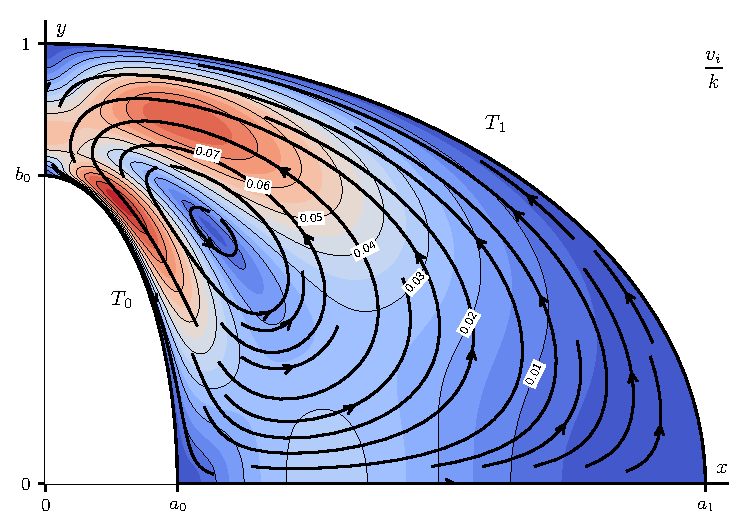
\includegraphics[width=\linewidth]{{{elliptic/kgf-0.02-flow}}}
                \vspace{-20pt}
                \caption{уравнения КГФ с граничными условиями ведущего порядка}
            \onslide<2| handout:2>
                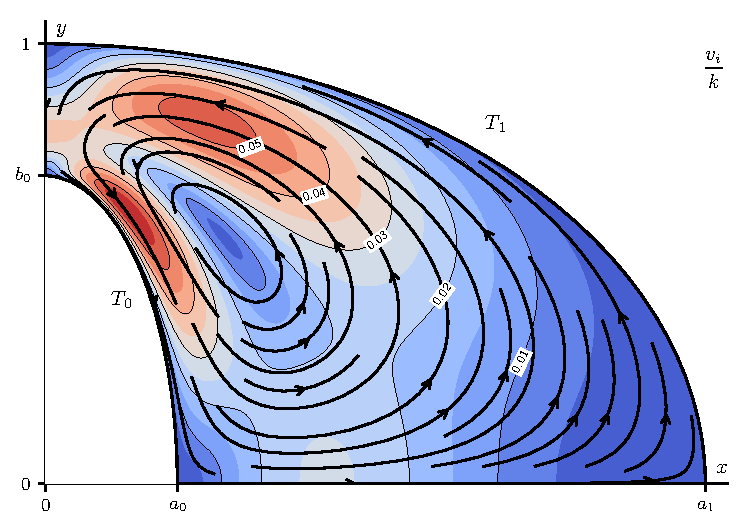
\includegraphics[width=\linewidth]{{{elliptic/first-0.02-flow}}}
                \vspace{-20pt}
                \caption{уравнения КГФ с граничными условиями первого порядка}
            \onslide<3| handout:1>
                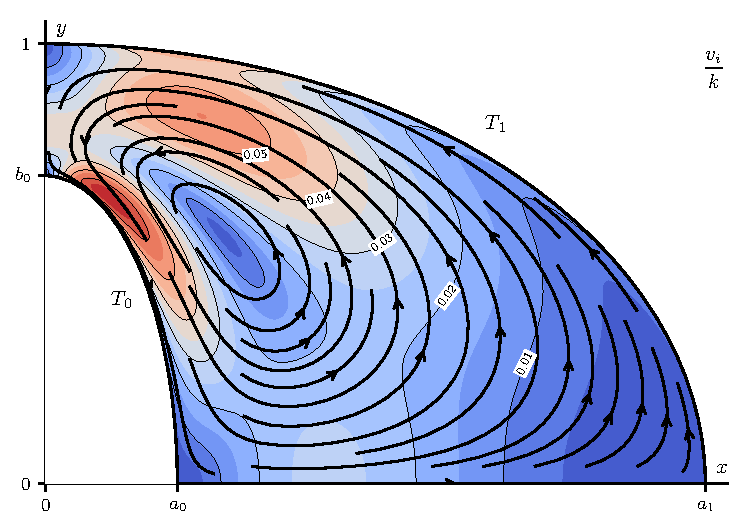
\includegraphics[width=\linewidth]{{{elliptic/second-0.02-flow}}}
                \vspace{-20pt}
                \caption{уравнения КГФ с граничными условиями второго порядка}
            \onslide<4| handout:0>
                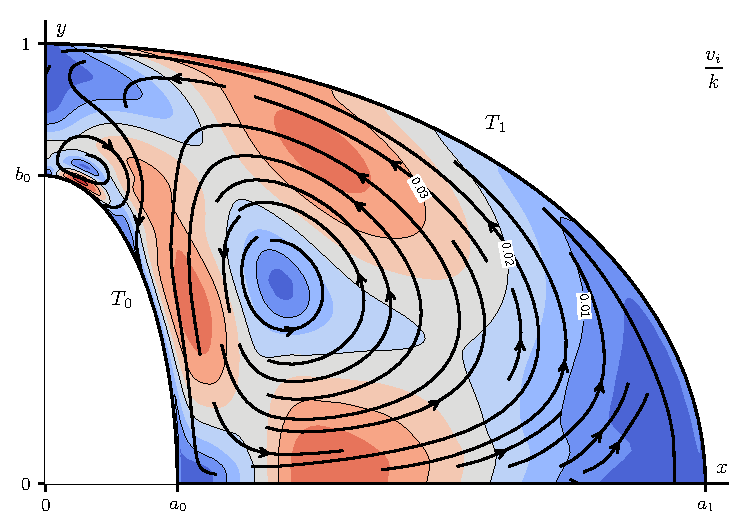
\includegraphics[width=\linewidth]{{{elliptic/kes-0.02-flow}}}
                \vspace{-20pt}
                \caption{численное решение уравнения Больцмана}
        \end{overprint}
    \end{figure}
\end{frame}

\begin{frame}
    \frametitle{Заключение}
    \begin{itemize}
        \item Прикладные области: MEMS, нелинейный термофорез, пожары на космических станциях.
        \item Гидродинамическое описание газа может оказаться некорректным на масштабах существенно больше длины свободного пробега,
        если градиенты макроскопических величин в некоторых областях сравнимы с обратным числом Кнудсена.
    \end{itemize}
\end{frame}



\end{document}
